\documentclass[11pt]{amsart}
\usepackage{geometry}                % See geometry.pdf to learn the layout options. There are lots.
\geometry{letterpaper}                   % ... or a4paper or a5paper or ... 
%\geometry{landscape}                % Activate for for rotated page geometry
%\usepackage[parfill]{parskip}    % Activate to begin paragraphs with an empty line rather than an indent
\usepackage{graphicx}
\usepackage{amssymb}
\usepackage{epstopdf}
\usepackage[usenames,dvipsnames]{color}
\usepackage{fancyvrb}
\usepackage{listings}
\usepackage{booktabs,footmisc}
\usepackage{hyperref}
\usepackage[all]{hypcap}

\usepackage{topcapt}


 
% include the lines below to use a nicer fixed-width font than the default one
 
\lstset{fancyvrb=true}
\lstset{
	basicstyle=\small\tt,
	identifierstyle=,
	commentstyle=\color{Bittersweet},
	stringstyle=\color{red},
	showstringspaces=false,
	tabsize=3,
	numbers=left,
	captionpos=b,
	xleftmargin=2em
%	numberstyle=\tiny
	%stepnumber=4
	}
\DeclareGraphicsRule{.tif}{png}{.png}{`convert #1 `dirname #1`/`basename #1 .tif`.png}

\title{Repast Model Testing Guide}
\author{Jonathan Ozik, Nick Collier - Repast Development Team}
\date{\today}                                           % Activate to display a given date or no date

\begin{document} 
\maketitle
\setcounter{section}{-1}

\section{Before we Get Started}
Before we can do anything with Repast Simphony, we need to make sure that we have a proper installation of Repast Simphony 2.1. Instructions on downloading and installing Repast Simphony on various platforms can be found on the \href{http://repast.sourceforge.net/download.html}{Repast website}.

\section{Getting Started with Repast Simphony Model Testing}

This guide will walk you through a few model testing use cases using Repast Simphony. To learn more about model testing, including the benefits of test driven development (TDD) when developing agent models, see Collier and Ozik (2013)\footnote{Collier, N, and J Ozik. �Test-Driven Agent-Based Simulation Development.� To appear in WSC 2013 Proceedings. Washington, D.C., 2013.}.

To add tests into an existing Repast Simphony project, we recommend the following setup steps:
\begin{enumerate}
\item
Add a \texttt{test} source folder to the project. This can be accomplished in a number of ways. One way is to right click on the project and navigate to \emph{New} $\rightarrow$ \emph{Source Folder} (Fig.~\ref{fig:newSourceFolder}). Then fill in \texttt{test} in the \emph{Folder name} text field and click on \emph{Finish} (Fig.~\ref{fig:testSourceFolder}).

\begin{figure}
\begin{center}
\vspace{.2in}
\centerline {
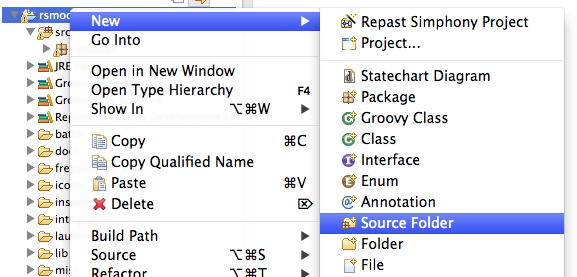
\includegraphics[width=4in]{RepastModelTestingImages/NewSourceFolder.png}
}
\caption{Selecting your project, right-clicking and choosing \emph{New} $\rightarrow$ \emph{Source Folder}.}
\label{fig:newSourceFolder}
\end{center}
\end{figure}

\begin{figure}
\begin{center}
\vspace{.2in}
\centerline {
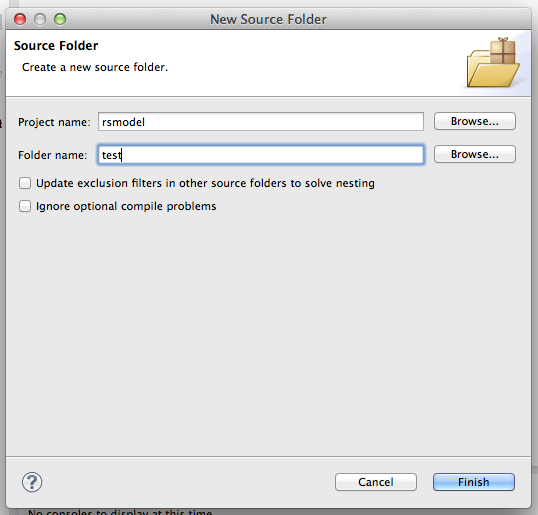
\includegraphics[width=4in]{RepastModelTestingImages/testSourceFolder.png}
}
\caption{New source folder wizard.}
\label{fig:testSourceFolder}
\end{center}
\end{figure}

\item
Modify the output folder for the \texttt{test} source folder. Right click on the project and navigate to \emph{Properties}. Then choose the \emph{Java Build Path} entry in the left bar and select the \emph{Source} tab. Select the check box that reads \emph{Allow output folders for source folders} and expand the \texttt{test} entry (Fig.~\ref{fig:javaBuildPath}). Select the \emph{Output folder} entry and click on the \emph{Edit} button (Fig.~\ref{fig:EditOutputFolder}). Then select the \textit{Specific output folder} option and input \texttt{testbin}, or something else different from \texttt{bin} (Fig.~\ref{fig:SourceFolderOutputLocation}). Click on \emph{Okay} and then \emph{Okay} again.

\begin{figure}
\begin{center}
\vspace{.2in}
\centerline {
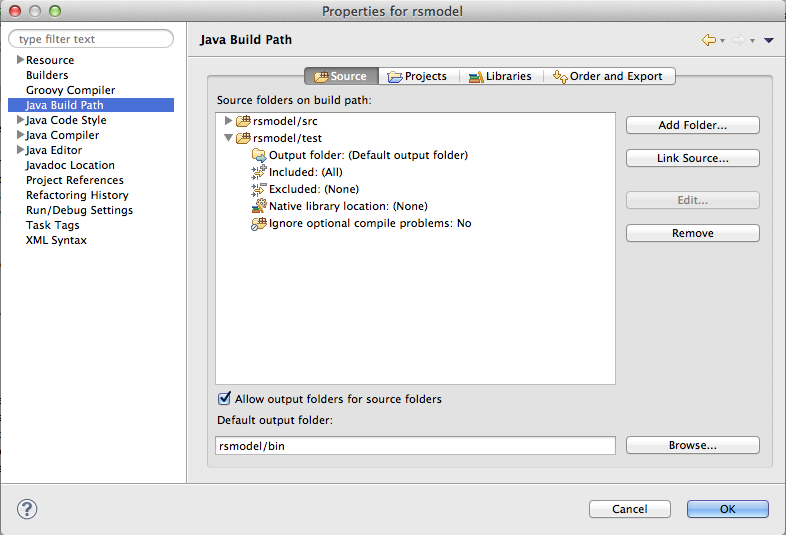
\includegraphics[width=4in]{RepastModelTestingImages/javaBuildPath.png}
}
\caption{\emph{Java Build Path} $\rightarrow$ \emph{Source} tab in a project's properties.}
\label{fig:javaBuildPath}
\end{center}
\end{figure}

\begin{figure}
\begin{center}
\vspace{.2in}
\centerline {
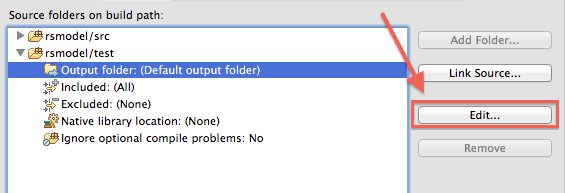
\includegraphics[width=4in]{RepastModelTestingImages/EditOutputFolder.png}
}
\caption{Edit the output folder of the \texttt{test} source folder.}
\label{fig:EditOutputFolder}
\end{center}
\end{figure}

\begin{figure}
\begin{center}
\vspace{.2in}
\centerline {
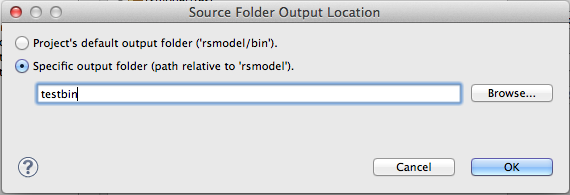
\includegraphics[width=4in]{RepastModelTestingImages/SourceFolderOutputLocation.png}
}
\caption{Choosing the source folder output location.}
\label{fig:SourceFolderOutputLocation}
\end{center}
\end{figure}


\item
Add a JUnit Test Case by right clicking on the project in the Package Explorer view,  choosing \emph{New} $\rightarrow$ \emph{Other}\ldots (Fig.~\ref{fig:newOther}). Then navigate to \emph{Java} $\rightarrow$ \emph{JUnit} and choose \emph{Junit Test Case} (Fig.~\ref{fig:JUnitTestCase}). In the \emph{New JUnit Test Case} wizard choose the \emph{New JUnit 4 test} option, specify the correct source folder (\texttt{test}), name your test case, include all the method stubs, and click on \emph{Finish} (Fig.~\ref{fig:NewJUnitTestCase}). If JUnit was not previously on your project's build path, you will see a dialog asking if you'd like to add it (Fig.~\ref{fig:AddToBuildPath}). Click \emph{OK} to add the JUnit 4 library to the project's build path.

\begin{figure}
\begin{center}
\vspace{.2in}
\centerline {
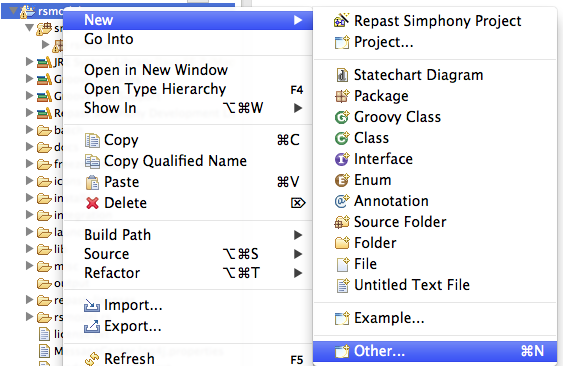
\includegraphics[width=4in]{RepastModelTestingImages/NewOther.png}
}
\caption{Selecting your project, right-clicking and choosing New $\rightarrow$ Other... .}
\label{fig:newOther}
\end{center}
\end{figure}

\begin{figure}
\begin{center}
\vspace{.2in}
\centerline {
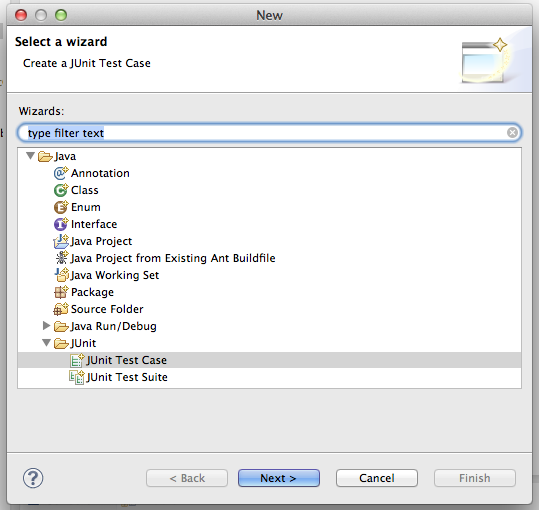
\includegraphics[width=3in]{RepastModelTestingImages/JUnitTestCase.png}
}
\caption{The JUnit Test Case option within Java $\rightarrow$ JUnit.}
\label{fig:JUnitTestCase}
\end{center}
\end{figure}

\begin{figure}
\begin{center}
\vspace{.2in}
\centerline {
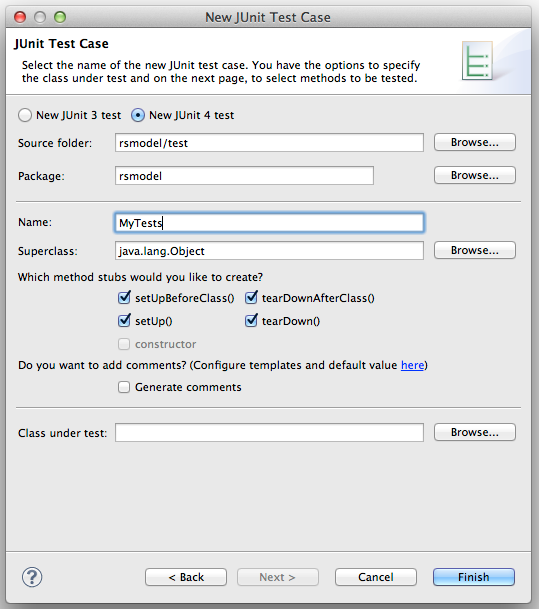
\includegraphics[width=3in]{RepastModelTestingImages/NewJUnitTestCase.png}
}
\caption{The new \emph{JUnit Test Case} wizard.}
\label{fig:NewJUnitTestCase}
\end{center}
\end{figure}

\begin{figure}
\begin{center}
\vspace{.2in}
\centerline {
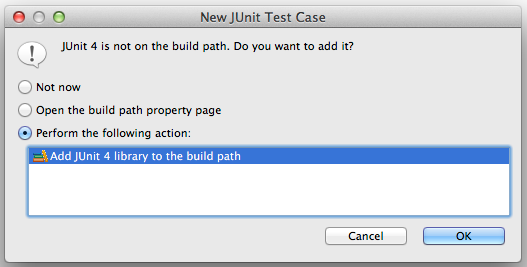
\includegraphics[width=4in]{RepastModelTestingImages/AddToBuildPath.png}
}
\caption{Add JUnit 4 library to build path.}
\label{fig:AddToBuildPath}
\end{center}
\end{figure}

\end{enumerate}
\clearpage

Once the setup is complete, there are a number of different types of model tests that can be created, based on the nature of the model behavior that is being tested. We will go over a few such cases next.

\subsection{Use Case 1: Simple Unit Testing with Repast Simphony Models}
If the elements being tested are relatively decoupled, there is nothing special that needs to be done in terms of test case setup. In this scenario, the @BeforeClass, @AfterClass, @Before, and @After annotated methods do not need any Repast Simphony specific elements and tests can be written in the usual way JUnit tests are written.

\subsection{Use Case 2: Schedule Based Model Testing with Repast Simphony Models}

\noindent\begin{minipage}[h]{\textwidth}
\vspace{.2in}
\lstset{language=java,caption=@Setup method in a schedule dependent test case.,label=lst:scheduleSetup}
\begin{lstlisting}
@Before
public void setUp() throws Exception {
	Schedule schedule = new Schedule();
	RunEnvironment.init(schedule, null, null, true);
	Context context = new DefaultContext();
	RunState.init().setMasterContext(context);
	
	// Any additional setup
}

\end{lstlisting}
\vspace{.2in}
\end{minipage}


\subsection{Use Case 3: Context Builder Based Model Testing with Repast Simphony Models}
For cases

\noindent\begin{minipage}[h]{\textwidth}
\vspace{.2in}
\lstset{language=java,caption=@Setup method in a schedule dependent test case.,label=lst:scheduleSetup}
\begin{lstlisting}
. . .
public Context context;

@Before
public void setUp() throws Exception {
	Schedule schedule = new Schedule();
	RunEnvironment.init(schedule, null, null, true);
	context = new DefaultContext();
	MyContextBuilder builder = new MyContextBuilder();
	context = builder.build(context);
	RunState.init().setMasterContext(context);
	
	// Any additional setup
}
. . .
\end{lstlisting}
\vspace{.2in}
\end{minipage}


\subsection{Use Case 4: Model Testing with ReLogo Models}
For cases

\noindent\begin{minipage}[h]{\textwidth}
\vspace{.2in}
\lstset{language=java,caption=@Setup method in a schedule dependent test case.,label=lst:scheduleSetup}
\begin{lstlisting}
. . .
static UserObserver observer;

@BeforeClass
public static void setUpBeforeClass() throws Exception {
	String scenarioDirString = "ModelName.rs"
	File paramsFile = new File(new File(scenarioDirString),
	          "parameters.xml");
	ParametersParser pp = new ParametersParser(paramsFile);
	Parameters params = pp.getParameters();
	RunEnvironment.init(new Schedule(), null, params, true);
	Context context = new DefaultContext();
	SimBuilder builder = new SimBuilder();
	context = builder.build(context);
	observer = (UserObserver) context.iterator().next();
	
	// Any additional before class setup
}

@Before
public void setUp() throws Exception {
	observer.clearAll();

	// Any additional setup
}
. . .
\end{lstlisting}
\vspace{.2in}
\end{minipage}

%Steps for creating harness: 
%create test source folder 
%output folder testbin 
%new package newproject.relogo in test source folder 
%new JUnit 4 test with all options checked (i.e., @BeforeClass, etc.) 
%
%Two examples to the right, one Java one Groovy. 
%Both can accept an "rsFolder" system property, e.g.: 
%
%-DrsFolder=${workspace_loc:NewProject}/NewProject.rs 
%
%Tried Spock but the dependencies weren�t convenient.


\end{document}  